% Quantum PINN architecture and physics-informed loss; adapted from Figure 1 of the article.
% Render both themes using: bash src/diagrams/render.sh
\documentclass[tikz,border=0pt]{standalone}
\usepackage[T1]{fontenc}
\usepackage{newtxtext,newtxmath}
\usepackage{amsmath}
\usetikzlibrary{arrows.meta,positioning,calc,fit,backgrounds}
\ifdefined\darkmode
  \definecolor{canvas}{HTML}{0D1117}
  \definecolor{ink}{HTML}{E6EDF3}
  \definecolor{muted}{HTML}{9198A1}
  \definecolor{network}{HTML}{1B2B44}
  \definecolor{networkline}{HTML}{79B8FF}
  \definecolor{output}{HTML}{2A2340}
  \definecolor{outputline}{HTML}{B392F0}
  \definecolor{autodiff}{HTML}{3A2A1A}
  \definecolor{autodiffline}{HTML}{F0B072}
  \definecolor{physics}{HTML}{16302A}
  \definecolor{physicsline}{HTML}{56D4A6}
  \definecolor{loss}{HTML}{3A1F28}
  \definecolor{lossline}{HTML}{F28BA8}
\else
  \definecolor{canvas}{HTML}{FFFFFF}
  \definecolor{ink}{HTML}{1F2328}
  \definecolor{muted}{HTML}{59636E}
  \definecolor{network}{HTML}{DDEBF7}
  \definecolor{networkline}{HTML}{0B5CAD}
  \definecolor{output}{HTML}{ECECFA}
  \definecolor{outputline}{HTML}{5A3FA8}
  \definecolor{autodiff}{HTML}{FDE8D0}
  \definecolor{autodiffline}{HTML}{A35A00}
  \definecolor{physics}{HTML}{E3F4E5}
  \definecolor{physicsline}{HTML}{1E7A3C}
  \definecolor{loss}{HTML}{FFEFF1}
  \definecolor{lossline}{HTML}{B3261E}
\fi
\begin{document}
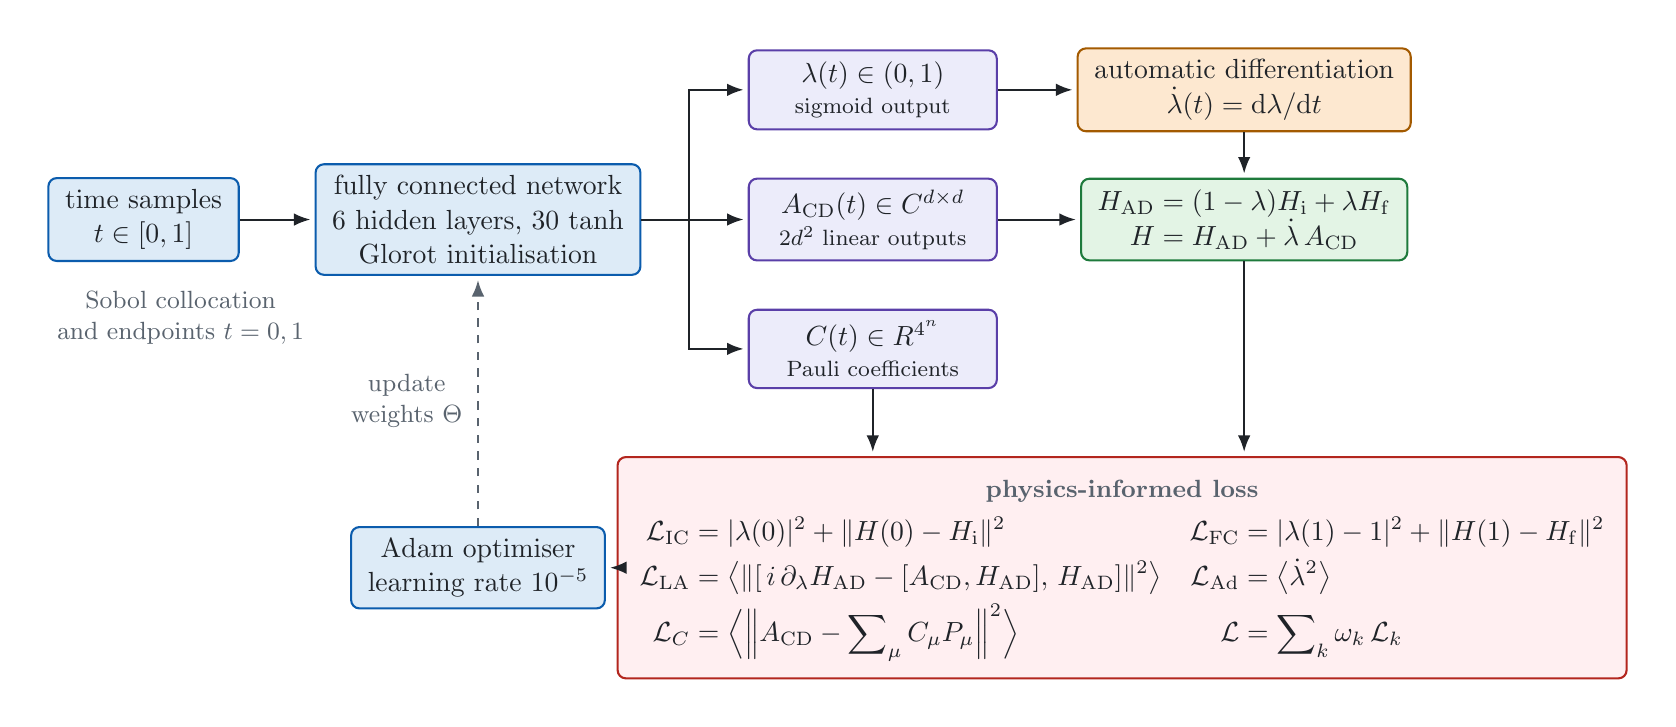
\begin{tikzpicture}[
  font=\fontsize{10}{12.5}\selectfont, text=ink,
  flow/.style={-{Latex[length=2.1mm,width=1.6mm]},draw=ink,line width=.75pt,
    shorten >=1.5pt},
  trunk/.style={draw=ink,line width=.75pt},
  feedback/.style={-{Latex[length=2.1mm,width=1.6mm]},draw=muted,line width=.75pt,
    dashed,shorten >=1.5pt},
  block/.style={rounded corners=3pt,line width=.75pt,align=center,inner xsep=6pt,
    inner ysep=4pt,minimum height=1.0cm},
  netbox/.style={block,draw=networkline,fill=network},
  outbox/.style={block,draw=outputline,fill=output,minimum width=3.15cm,minimum height=.9cm},
  autobox/.style={block,draw=autodiffline,fill=autodiff},
  physbox/.style={block,draw=physicsline,fill=physics},
  lossbox/.style={block,draw=lossline,fill=loss,inner xsep=8pt,inner ysep=6pt},
  title/.style={font=\fontsize{9}{11}\selectfont\bfseries,text=muted,anchor=south west},
  note/.style={font=\fontsize{9}{11}\selectfont,text=muted,align=center}
]
% --- Forward pass ---------------------------------------------------------------
\node[netbox,minimum width=2.4cm] (time) at (0,0) {time samples\\$t\in[0,1]$};
\node[netbox,minimum width=3.0cm,right=0.95cm of time] (network)
  {fully connected network\\6 hidden layers, 30 tanh\\Glorot initialisation};
\node[outbox,right=1.35cm of network] (A) {$A_{\mathrm{CD}}(t)\in\mathbb{C}^{d\times d}$\\[-1pt]
  {\fontsize{8.5}{10}\selectfont $2d^2$ linear outputs}};
\node[outbox,above=0.6cm of A] (lambda) {$\lambda(t)\in(0,1)$\\[-1pt]
  {\fontsize{8.5}{10}\selectfont sigmoid output}};
\node[outbox,below=0.6cm of A] (C) {$C(t)\in\mathbb{R}^{4^{n}}$\\[-1pt]
  {\fontsize{8.5}{10}\selectfont Pauli coefficients}};
\node[autobox,right=1.0cm of lambda,minimum width=3.6cm] (autodiff)
  {automatic differentiation\\$\dot\lambda(t)=\mathrm{d}\lambda/\mathrm{d}t$};
\node[physbox,minimum width=3.6cm] (H) at (autodiff.center |- A.center)
  {$H_{\mathrm{AD}}=(1-\lambda)H_{\mathrm{i}}+\lambda H_{\mathrm{f}}$\\
   $H=H_{\mathrm{AD}}+\dot\lambda\,A_{\mathrm{CD}}$};

\draw[flow] (time.east) -- (network.west);
\coordinate (split) at ($(network.east)+(0.6,0)$);
\draw[trunk] (network.east) -- (split);
\draw[flow] (split) |- (lambda.west);
\draw[flow] (split) -- (A.west);
\draw[flow] (split) |- (C.west);
\draw[flow] (lambda.east) -- (autodiff.west);
\draw[flow] (autodiff.south) -- (H.north);
\draw[flow] (A.east) -- (H.west);

% --- Loss --------------------------------------------------------------------------
\node[lossbox,anchor=north] (loss) at ($(H.south |- C.south)+(-1.55,-0.85)$) {%
  \begin{tabular}{@{}c@{}}
  {\fontsize{9}{11}\selectfont\bfseries\color{muted} physics-informed loss}\\[3pt]
  $\begin{aligned}
    \mathcal{L}_{\mathrm{IC}}&=|\lambda(0)|^2+\lVert H(0)-H_{\mathrm{i}}\rVert^2 &
    \mathcal{L}_{\mathrm{FC}}&=|\lambda(1)-1|^2+\lVert H(1)-H_{\mathrm{f}}\rVert^2\\
    \mathcal{L}_{\mathrm{LA}}&=\bigl\langle\lVert[\,i\,\partial_\lambda H_{\mathrm{AD}}
      -[A_{\mathrm{CD}},H_{\mathrm{AD}}],\,H_{\mathrm{AD}}]\rVert^2\bigr\rangle &
    \mathcal{L}_{\mathrm{Ad}}&=\bigl\langle\dot\lambda^2\bigr\rangle\\
    \mathcal{L}_{C}&=\Bigl\langle\Bigl\lVert A_{\mathrm{CD}}-\sum\nolimits_\mu C_\mu P_\mu
      \Bigr\rVert^2\Bigr\rangle &
    \mathcal{L}&=\sum\nolimits_k\omega_k\,\mathcal{L}_k
  \end{aligned}$
  \end{tabular}};
\draw[flow] (H.south) -- (H.south |- loss.north);
\draw[flow] (C.south) -- (C.south |- loss.north);

\node[netbox,minimum width=3.0cm] (adam) at (network.center |- loss.center)
  {Adam optimiser\\learning rate $10^{-5}$};
\draw[flow] (loss.west) -- (adam.east);
\draw[feedback] (adam.north) -- (network.south)
  node[midway,left,note,xshift=-2pt] {update\\weights $\Theta$};

\node[note,anchor=north west] at ($(time.south west)+(0,-0.25)$)
  {Sobol collocation\\and endpoints $t=0,1$};

\begin{scope}[on background layer]
  \fill[canvas] ($(current bounding box.south west)+(-0.25,-0.25)$)
    rectangle ($(current bounding box.north east)+(0.25,0.25)$);
\end{scope}
\end{tikzpicture}
\end{document}
